\appendix

\section{Implementation Details}\label{appendix:implementation_details}


\subsection{Rewards and Constraints}

We use the reward function~\ref{eq:rew_lin_vel} from~\citep{cheng2023parkour} that measures progress toward a specific direction.
To always have positive rewards, we add a survival bonus of $0.5$ at each time step, and, following~\citep{rudin2022learning}, we clip total rewards below $0.0$.

To enforce the constraints, we follow CaT~\citep{chane2024cat} and reformulate the constrained RL problem~\ref{eq:mdp} into the following RL problem:
\begin{equation}
\max_\pi \underset{\tau \sim \pi}{\mathbb{E}} \! \left [ \sum_{t=0}^\infty \! \left ( \prod_{t'=0}^t \gamma (1 - \delta (s_{t'}, a_{t'})) \! \right ) \! r(s_t, a_t) \right ], 
\label{eq:cat_mdp}
\end{equation}
with termination probabilities $\delta(s_t, a_t)$.
Following CaT, we define the termination probabilities as:
\begin{equation}
\label{eq:delta_function}
\delta = \max_{i \in I} \: p_i^\text{max} \text{clip}(\frac{c_i^+}{c_i^\text{max}}, 0, 1),
\end{equation}
where $c_i^+ = \max(0, c_i(s, a))$ is the violation of constraint $i$, $c_i^\text{max}$ is an exponential moving average of the maximum constraint violation over the last batch of experience collected in the environment, and $p_i^\text{max}$ a hyperparameter that controls the maximum termination probability for the constraint $i$.

Table~\ref{table:constraint_list} lists all the constraints used.
Following~\citep{chane2024cat}, we separate constraints between hard constraints, where $p_i^\text{max}=1.0$, and soft constraints, where $p_i^\text{max}$ increases throughout the course of training, allowing the RL agent to discover agile locomotion during the early stage of training while enforcing more the constraints later on to ensure safe behaviors.
To encourage the emergence of a specific locomotion style, some constraints are activated only in specific settings.
For instance, the \textit{Stand still} constraints $c_\text{still}$ are only active when no velocity command is provided, whereas the \textit{Base orientation} and \textit{Number of foot contacts} are only active on flat terrains and on early terrain levels. 
We found that rescaling the constraint violations by the square root function $c_i \leftarrow \sqrt{c_i^+}$ helps CaT be less sensitive to extreme values of constraint violations.

\begin{table}[h]
\centering
\begin{tabular}{c|c|c|c}
\toprule
Type & Expression & Hard & Cond. \\
\midrule
Knee or base collision & $c_\text{knee/base contact} = 1_\text{knee/base contact}$ & $\checkmark$ & $\times$ \\
Foot contact force & $c_{\text{foot contact}_j} = \|f^{\text{foot}_j}\|_2 - f^\text{lim}$  & $\checkmark$ & $\times$ \\
Foot stumble  & $c_{\text{stumble}_j} = \|f^{\text{foot}_j}_\text{xy}\|_2 - 4 |f^{\text{foot}_j}_\text{z}|$ & $\times$ & $\times$ \\
Heading  & $c_{\text{heading}} = |\text{angle}_\text{base} - \text{angle}_\text{cmd}| - \text{angle}^\text{lim} $ & $\times$ & $\times$ \\
Torque  & $c_{\text{torque}_k} = |\tau_k| - \tau^\text{lim}$ & $\times$ & $\times$ \\
Joint velocity  & $c_{\text{joint velocity}_k}= |\dot{q_k}| - \dot{q}^\text{lim}$  & $\times$ & $\times$ \\
Joint acceleration & $c_{\text{joint acceleration}_k}= |\ddot{q_k}| - \ddot{q}^\text{lim}$ & $\times$ & $\times$ \\
Action rate  & $c_{\text{action rate}_k}= \frac{\left | \Delta q^\text{des}_{t, k} - \Delta q^\text{des}_{t-1, k} \right |}{dt} - \dot{q}^\text{des lim}$ & $\times$ & $\times$ \\

Joint limits min & $c_{\text{join}^\text{min}_j} = \text{joint}^\text{min}_j - \text{joint}_j$ & $\times$ & $\times$ \\
Joint limits max & $c_{\text{join}^\text{max}_j} =  \text{joint}_j - \text{joint}^\text{max}_j$ & $\times$ & $\times$ \\
Foot air time & $c_{\text{air time}_j} = t_\text{air time}^\text{des} - t_{\text{air time}_j}$ & $\times$ & $\times$ \\
Base orientation (roll-axis) & $c_{\text{ori}_\text{roll}} = | \text{ori}_\text{roll} | - \text{ori}^\text{lim}_\text{roll}$ & $\times$ & $\times$ \\
Base orientation & $c_\text{ori} = \left \| \text{base ori}_{\text{xy}} \right \|_2 - \text{base}^\text{lim}$ & $\times$ & $\checkmark$ \\
Number of foot contacts & $c_\text{n foot contacts} = |n_\text{foot contact} - n_\text{foot contact}^\text{des}|$ & $\times$ & $\checkmark$  \\
Stand still & $c_{\text{still}}= \|q - q^\star \|_2 - \epsilon_\text{still}$ & $\times$ & $\checkmark$ \\
\bottomrule
\end{tabular}
\vspace{0.3cm}
\caption{List of constraints, where \textit{Hard} indicates whether each row corresponds to a hard constraint and \textit{Cond.} indicates whether a constraint is active only under certain conditions.}
\label{table:constraint_list}
\end{table}

\subsection{Policy Learning}
\label{appendix:policy_learning}

We built our RL algorithm with the CleanRL~\citep{huang2022cleanrl} implementations of PPO and DDPG.
During privileged policy learning, we linearly increase the damping parameter (Kd) of the PD controller from $0.05$ to $0.2$ but keep it fixed at $0.2$ during visual policy learning.
Indeed, we empirically observed that RL discovers agile skills more easily with lower Kd but policies with higher Kd transfer better to the real Solo-12.


\paragraph{Privileged Policy Learning}
An MLP parametrizes the privileged policy with hidden dimensions $[512, 256, 128]$ and elu activations.
We use PPO~\citep{schulman2017proximal} with $4096$ actors in parallel in simulation.
The training procedure is very similar to~\citep{rudin2022learning, cheng2023parkour, chane2024cat}. 


\paragraph{Visual Policy Learning}
The actor processes depth images using a vision neural network consisting of three blocks of a convolution with leaky ReLU activations, followed by max pooling and a linear layer to produce the depth embeddings.
Random translation, random noise, and random cutout are applied to the depth images during training.
The actor then processes the history of proprioceptive information, actions, and depth embeddings with a one-layer Gated Recurrent Unit~\citep{chung2014empirical} (GRU) of hidden size 256.
This GRU is followed by a MLP with hidden dimensions $[512, 256, 128]$ and elu activations.
The output of the final layer is processed by a tanh activation function and rescaled to produce the 12-dimensional action vector.
We used the action bounds observed in the privileged experience buffer to rescale the actions given by the actor.

The critic network is parameterized by a MLP with hidden dimensions $[512, 256, 128]$, layer normalization and elu activations.
While the actor observes the full state $s_t$, which includes a history of depth images, the critics process the privileged state $s_t^\text{priv}$, which includes privileged heightmap scan and ceilings instead of high-dimensional images.

We generate trajectories from the privileged policy that amounts to 2 million state-action samples and store them in the privileged experience buffer $\mathcal{D}^\text{priv}$ whereas online experience is collected by $256$ actors in parallel into the online replay buffer $\mathcal{D}^\text{online}$.
We store the constraint violations $c_i^+$ of both online and privileged experience in their respective replay buffers to recompute the termination probabilities $\delta$ on the fly during off-policy learning.
Both $\mathcal{D}^\text{priv}$ and  $\mathcal{D}^\text{online}$ store privileged information at every step and depth image every 5 environment steps.
During training, we only give the vision network one image every five timesteps and then replicate the depth latent five times to match the sequence length of the other observations. 
The online replay buffer stores the GRU hidden latent produced by the online actors whereas the privileged replay buffer stores zeros for these latents.
This is done to initialize the first hidden of the DDPG actor correctly during off-policy training.

We train the visual policy using a variant of RLPD~\citep{ball2023efficient}.
We build upon DDPG~\citep{lillicrap2015continuous} with an update-to-data ratio of $8$ during policy evaluation.
We use REDQ~\citep{chen2021randomized} with 10 critics and an ensemble of 2 random critic targets.


\subsection{Baselines}

The BC baseline uses the same neural network architecture as SoloParkour, as described in Section \ref{appendix:policy_learning}.
We train the BC policies to regress the action based on the history of observations on the same dataset of demonstrations $\mathcal{D}^\text{priv}$ generated by the privileged policy $\pi^\text{priv}$ as SoloParkour.

The DAgger baseline uses the same neural network architecture as SoloParkour and BC.
We employ the Stage 1 policy $\pi^\text{priv}$ as teacher for action relabelling.
We found that starting the DAgger policy from the BC-pretrained weights greatly improves online learning efficiency.

For the \textit{Privileged Reconstruction} baseline, we use the same observation space and neural architecture as SoloParkour, BC and DAgger for the vision module except that the output of the GRU is projected to the privileged information space through a linear layer.
We employ the privileged policy $\pi^\text{priv}$ as frozen MLP head and only train the vision module to reconstruct the privileged information from the history of past observations and actions.
Similar to~\citep{agarwal2023legged} and unlike~\citep{duan2023learning}, we found it highly beneficial to train the vision network with experience generated by the resulting online policy, rather than training solely on the fixed dataset $D^\text{priv}$ generated by the privileged policy.


The \textit{No Priv. Critic} ablation processes visual input in the critic network instead of privileged information.
Its vision module follows the same architecture as the visual policy.

For the \textit{Visual RL w/o CaT} ablation, we use the same dataset of privileged experience $\mathcal{D}^\text{priv}$ as the one used to train all other methods (except for the \textit{From Scratch} ablation that doesn't learn from any demonstration), but we remove the constraints for Stage 2 RL.
Note that the privileged experience $\mathcal{D}^\text{priv}$ was generated with $\pi^\text{priv}$ which was trained with Constrained RL and therefore satisfies the constraints.



\section{Real Robot Setup}
We use the Solo-12 quadruped robot for our experiments.
We built a custom 3D-printed plastic piece to mount the Intel RealSense D405 stereo camera observing in front of the robot.
We use the Python wrapper of librealsense to capture depth images at resolution $424 \times 240$.
We resize and crop the images to $48 \times 48$ and apply the librealsense postprocessing hole-filling filter.
Depth images are preprocessed in a separate thread on a separate CPU as they come, at around 30Hz.
The visual policy runs at 50Hz using ONNX and produces target joint angles to torque by a PD controller with stiffness $Kp=4.0$ and damping $Kd=0.2$ running at $10$KHz.
Hence, depth embeddings are updated at a higher frequency at inference than during training.
All the computation is done through Python scripts by the onboard Raspberry Pi 5. 
Velocity commands are sent to the embedded controller via a wireless gamepad.


\section{Additional Results}
\label{appendix:additional_results}


In Figure \ref{fig:additional_constraints_1} and \ref{fig:additional_constraints_2}, we present further results on constraint satisfaction for SoloParkour and the baselines introduced in Section \ref{sec:experiments:setup}.
SoloParkour demonstrates high constraint satisfaction, highlighting the effectiveness of our approach in achieving safe yet agile locomotion skills over challenging terrains using vision.



\begin{figure}[h]
    \centering
    \begin{subfigure}[b]{\textwidth}
        \centering
        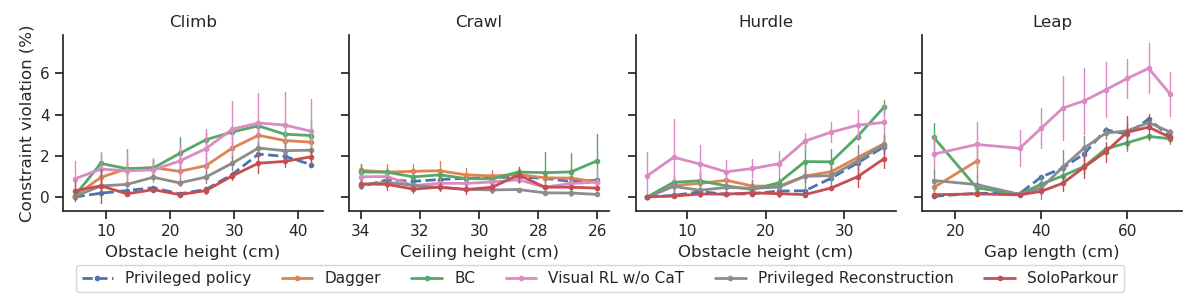
\includegraphics[width=\textwidth]{Assets/Results/torque1_exceeding.png}
        \caption{Torque constraint for the front left shoulder joint}
    \end{subfigure}
    \begin{subfigure}[b]{\textwidth}
        \centering
        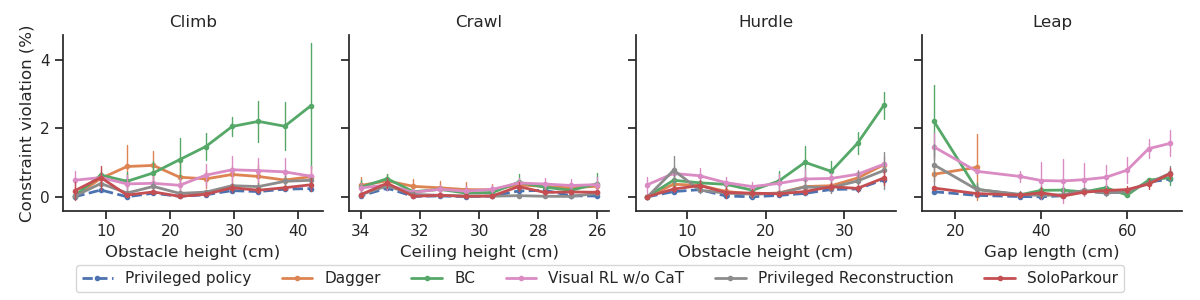
\includegraphics[width=\textwidth]{Assets/Results/vel2_exceeding.png}
        \caption{Joint velocity constraint for the front left knee}
    \end{subfigure}
    \begin{subfigure}[b]{\textwidth}
        \centering
        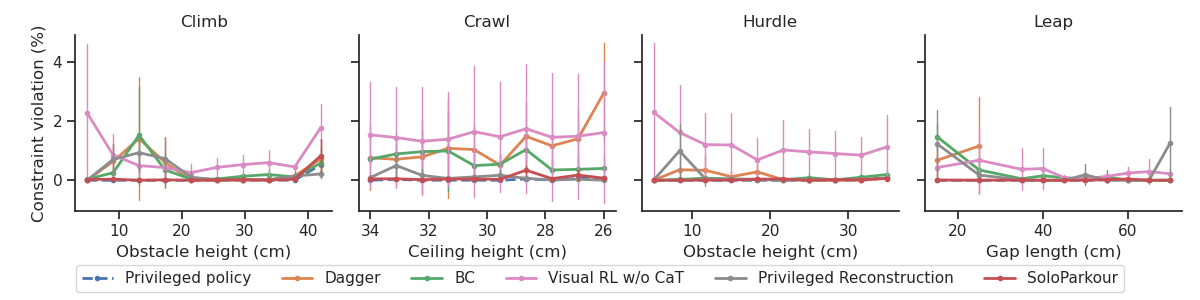
\includegraphics[width=\textwidth]{Assets/Results/HFE0_exceeding.png}
        \caption{Joint limit max constraint for the front left shoulder}
    \end{subfigure}
    \begin{subfigure}[b]{\textwidth}
        \centering
        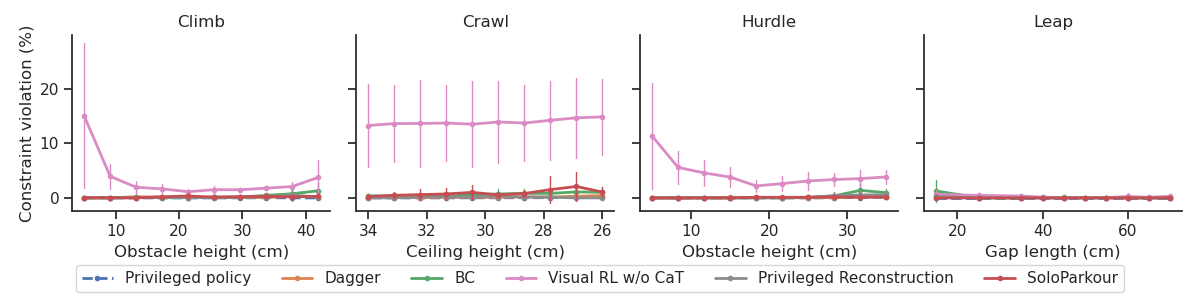
\includegraphics[width=\textwidth]{Assets/Results/KFE_min0_exceeding.png}
        \caption{Joint limit min constraint for the front left knee}
    \end{subfigure}
    
    \caption{Constraint violations (in \%) when the policies successfully traverse the terrain level by obstacle dimension, averaged across 4 training seeds.}
    \label{fig:additional_constraints_1}
    
\end{figure}

\begin{figure}[h]
    \centering
    \begin{subfigure}[b]{\textwidth}
        \centering
        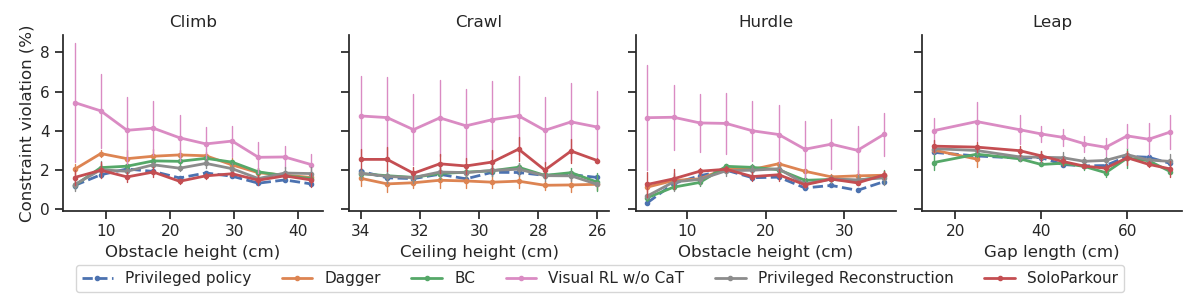
\includegraphics[width=\textwidth]{Assets/Results/air_time3_exceeding.png}
        \caption{Air time constraint for the hind right foot}
    \end{subfigure}
    \begin{subfigure}[b]{\textwidth}
        \centering
        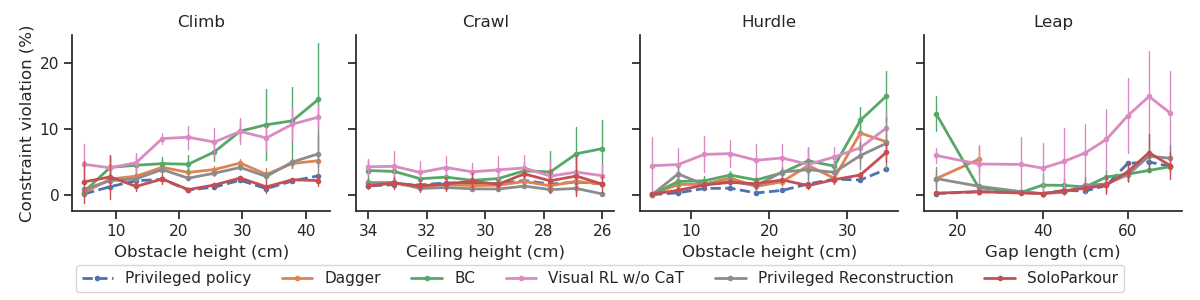
\includegraphics[width=\textwidth]{Assets/Results/heading0_exceeding.png}
        \caption{Heading constraint between the direction of the robot and the commanded direction}
    \end{subfigure}

    \begin{subfigure}[b]{\textwidth}
        \centering
        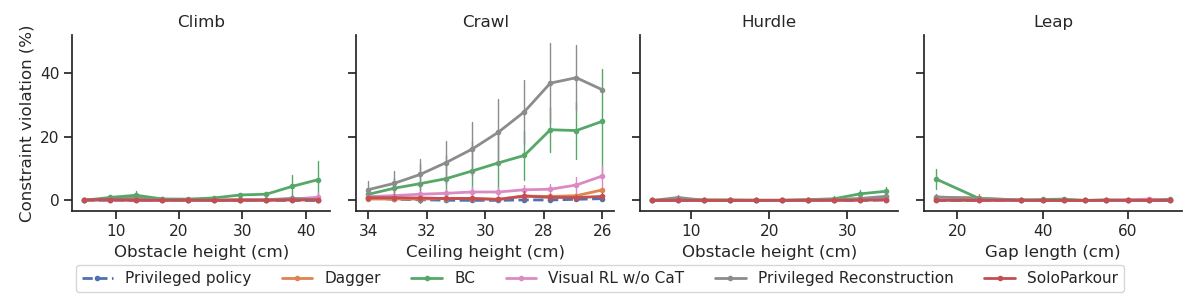
\includegraphics[width=\textwidth]{Assets/Results/base_contact0_exceeding.png}
        \caption{Collision constraint for the base of the robot}
    \end{subfigure}
    \begin{subfigure}[b]{\textwidth}
        \centering
        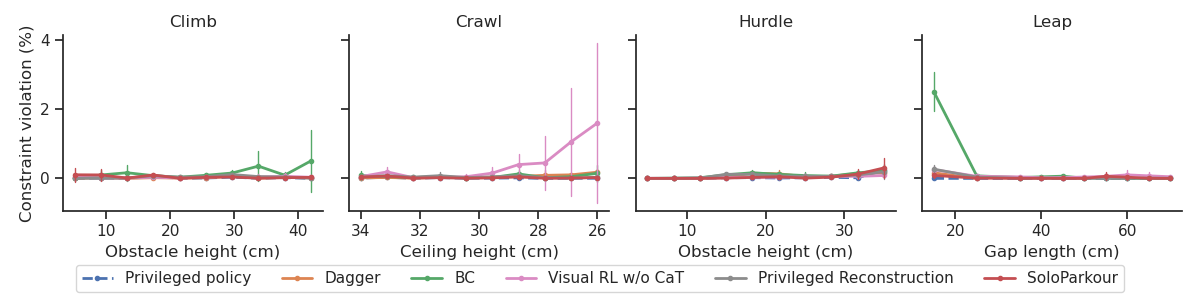
\includegraphics[width=\textwidth]{Assets/Results/knee_contact2_exceeding.png}
        \caption{Collision constraint for the hind left knee}
    \end{subfigure}
    
    \caption{Constraint violations (in \%) when the policies successfully traverse the terrain level by obstacle dimension, averaged across 4 training seeds.}
    \label{fig:additional_constraints_2}
    
\end{figure}